% Main chapter title
\chapter{Mathematische Grundlagen}

% Chapter label
\label{fundamentals}

In diesem Kapitel werden wir die wichtigsten mathematischen Grundlagen, die wir für die Formulierung der dünnbesetzten Hauptkomponentenanalyse benötigen, einführen. Dazu beschäftigen wir uns zunächst mit Grundbegriffen aus des linearen Algebra, Matrixzerlegungen und ausgewählten Approximationsproblemen in Abschnitt \ref{linear_algebra}. Ein Großteil dieses Kapitel ist linearen Regressionsmodellen gewidmet, welche wir mit verschiedenen Straftermen versehen werden, um gewisse Effekte zu erzielen. Anhand eines Beispiel-Datensatzes werden wir in der Lage sein, diese Effekte visuell nachzuvollziehen. Für den weiteren Verlauf dieser Arbeit ist das Verständnis der Strafterme von entscheidender Bedeutung. Zu Schluss werden wir in Abschnitt \ref{signal_processing} Grundlagen der Signalverarbeitung ausarbeiten, da wir in Kapitel \ref{application} die dünnbesetzte Hauptkomponentenanalyse auf Frequenzdaten anwenden.



%----------------------------------------------------------------------------------------
%	Lineare Algebra
%----------------------------------------------------------------------------------------



\section{Lineare Algebra}
\label{linear_algebra}

Ein Großteil der Mathematik der Hauptkomponentenanalyse beruht auf Methoden der linearen Algebra. Aufgrund des Anwendungsfalls werden wir uns auf die Einführung der Grundbegriffe in reellen Vektorräumen beschränken.

\subsection{Orthogonalität}
\label{orthogonality}

\begin{defn}[Skalarprodukt \cite{jaenich}]
Sei $V$ ein reeller Vektorraum. Ein \textit{Skalarprodukt} in $V$ ist eine Abbildung $\inner{\cdot}{\cdot}: V \times V \longrightarrow \mathbb{R}$ mit den folgenden Eigenschaften:
\begin{enumerate}[(i)]
\item Für jedes $x \in V$ sind die Abbildungen
\begin{align*}
\inner{\cdot}{x}: V & \longrightarrow \mathbb{R} & \inner{x}{\cdot}: V & \longrightarrow \mathbb{R}\\
v & \longmapsto \inner{v}{x} & v & \longmapsto \inner{x}{v}
\end{align*}
linear. $\quad$ (Bilinearität)
\item $\inner{x}{y} = \inner{y}{x}$ für alle  $x,y \in V \quad$ (Symmetrie)
\item $\inner{x}{x} > 0$ für alle $x \neq 0 \quad$ (Positive Definitheit)
\end{enumerate}
\end{defn}

Allgemein versteht man unter einem \textit{euklidischem Vektorraum} ein Paar $(V, \inner{\cdot}{\cdot})$, welches aus einem reellem Vektorraum $V$ und einem Skalarprodukt $\inner{\cdot}{\cdot}$ auf $V$ besteht. Durch das Skalarprodukt wird eine Norm auf $V$ induziert:
$$\norm{v} \defeq \sqrt{\inner{v}{v}}$$
In den folgenden Kapiteln werden wir uns vor allem mit dem \textit{Standardskalarprodukt} im $\mathbb{R}^n$ beschäftigen. Dies ist gegeben durch 
$$\inner{x}{y} = x_1y_1 + \cdots + x_ny_n.$$

\begin{thm}[Verallgemeinerter Satz des Pythagoras \cite{anton}]
\label{pythagoras}
Für orthogonale Vektoren $u,v$ in einem euklidischem Vektorraum $V$ gilt
$$\norm{u+v}^2 = \norm u^2 + \norm v^2.$$
\end{thm}

\begin{defn}[Orthogonalität \cite{jaenich}]
Zwei Elemente $v, w$ eines euklidischen Vektorraumes $V$ heißen \textit{orthogonal} (geschrieben $v \perp w$) wenn ihr Skalarprodukt null ist, d.h.
$$v \perp w \iff \inner{v}{w} = 0.$$
Eine Familie $(v_1, \ldots, v_n)$ in $V$ heißt \textit{orthogonal} oder \textit{Orthogonalsystem}, wenn
$$v_i \perp v_j \quad \text{für alle} \quad i \neq j.$$
Gilt zusätzlich $\inner{v_i}{v_i} = 1$ für alle $1 \leq i \leq n$, so spricht man von einem \textit{Orthonormalsystem}.
\end{defn}

%\begin{defn}[Orthonormalbasis \cite{fischer}]
%Sei $\inner{\cdot}{\cdot}: V \times V \longrightarrow \mathbb{R}$ ein Skalarprodukt. Ein System von Vektoren $(v_1, \ldots, v_n)$ in $V$ wird als \textit{Orthogonalbasis} (bzw. \textit{Orthonormalbasis}) bezeichnet, wenn folgende Bedingungen erfüllt sind:
%\begin{enumerate}[(i)]
%\item $(v_1, \ldots, v_n)$ ist eine Basis von $V$
%\item $(v_1, \ldots, v_n)$ ist ein Orthogonalsystem (bzw. Orthonormalsystem)
%\end{enumerate}
%\end{defn}

\begin{thm}[Existenz einer Orthonormalbasis \cite{fischer}]
Jeder endlichdimensionale euklidische Vektorraum besitzt eine Orthonormalbasis.
\end{thm}

Der Begriff der Orthogonalität lässt sich auf Matrizen übertragen.

\begin{defn}[Orthogonale Matrix \cite{anton}]
Eine Matrix $\mat A \in \mathbb{R}^{n \times n}$ heißt 		\textit{orthogonal}, falls deren Zeilen- und Spaltenvektoren paarweise orthonormal bezüglich des Standardskalarprodukts sind, d.h.
$$\mat A^{\top} \mat A = \mathbb{1}_n$$
\end{defn}

\begin{defn}[Orthogonalprojektion \cite{anton}]
Eine \textit{Orthogonalprojektion} auf einen Untervektorraum $U$ eines Vektorraumes $V$ ist eine lineare Abbildung $P_U \colon V \rightarrow V$, die für alle Vektoren $v \in V$ die beiden Eigenschaften
\begin{enumerate}[(i)]
\item $P_U(v) \in U \quad$ (Projektion)
\item $\langle P_U(v) - v , u \rangle = 0$ für alle $u \in U \quad$ (Orthogonalität)
\end{enumerate}
erfüllt.
\end{defn}

Mithilfe einer Orthogonalbasis für $U$ lässt sich aus dieser Definition eine Lösung für die Orthogonalprojektion $P_U(v)$ herleiten.

\begin{thm}[\cite{anton}]
\label{orthogonal_projection_theorem}
Ist $(u_1, \ldots, u_n)$ eine Orthogonalbasis von $U$, so gilt für alle $v \in V$
$$P_{U}(v) = \sum_{i=1}^n \frac{\langle v, u_i \rangle}{\langle u_i, u_i \rangle} u_i$$
\end{thm}

Später werden wir die Orthogonalprojektion in einer anderen Form nutzen. Wir können die Projektion auch als Matrix-Vektor-Produkt auffassen. Verwenden wir das Standardskalarprodukt gilt mit einer Orthogonalbasis $(u_1, \ldots, u_n)$ von $U$:
\begin{align}
P_U(v) = \sum_{i=1}^n \frac{v^{\top} u_i}{u_i^{\top} u_i} u_i = \sum_{i=1}^n \frac{u_i u_i^{\top}}{u_i^{\top} u_i}v = \mat A \mat A^{\top} v
\end{align}
wobei $\mat A = \begin{bmatrix} \frac{u_1}{\norm{u_1}} & \cdots & \frac{u_n}{\norm{u_n}} \end{bmatrix}$. Die Orthonormalitätsbedingung in Theorem \ref{orthogonal_projection_theorem} kann auch weggelassen werden. Ist $(u_{1},\ldots ,u_{n})$ eine beliebige Basis von $U$, so gilt:
\begin{align}
P_U(v) = \mat A (\mat A^\top \mat A)^{-1} \mat A^\top v
\end{align}
Wir nennen $\mat P = \mat A (\mat A^\top \mat A)^{-1} \mat A^\top$ die \textit{orthogonale Projektionsmatrix}. Mithilfe von Theorem \ref{pythagoras} lässt sich zeigen, dass der orthogonal auf den Unterraum projizierte Vektor den Abstand zwischen dem Ausgangsvektor und dem Unterraum minimiert.

\begin{thm}[\cite{anton}]
Sei $U$ ein Unterraum eines euklidischen Vektorraumes $V$. Dann ist $P_U(v)$ die beste Näherung von $u$ in $U$, d.h.
$$\norm{P_U(v) - v}^2 \leq \norm{u - v}^2 \quad \text{für alle } u \in U$$
\end{thm}


\subsection{Matrixzerlegungen}
\label{matrix_decomposition}

In diesem Abschnitt führen wir zwei wichtige Matrixzerlegungen ein, die auch in vielen Bereichen der Numerik Anwendung finden.

\begin{defn}[Eigenwert, Eigenvektor \cite{anton}]
Sei $\mat{A} \in \rnn$. Ein von Null verschiedener Vektor $x \in \rn$ heißt \textit{Eigenvektor} von $\mat{A}$, falls
$$\mat{A}x = \lambda x$$
für einen Skalar $\lambda \in \mathbb{R}$. Die Zahl $\lambda$ heißt \textit{Eigenwert} von $\mat{A}$.
\end{defn}

\begin{defn}[Diagonalisierbar \cite{anton}]
Eine quadratische Matrix $\mat A \in \rnn$ heißt \textit{diagonalisierbar}, wenn eine invertierbare Matrix $\mat V$ existiert, so dass $\mat{\Lambda} = \mat{V}^{-1}\mat{A}\mat{V}$ Diagonalgestalt hat.
\end{defn}

Es gibt verschiedene Kriterien für die Diagonalisierbarkeit von Matrizen. Für unsere spätere Anwendung interessieren wir uns vor allem für die Frage, ob es zu einer gegebenen Matrix $\mat{A} \in \rnn$ eine orthogonale Matrix $\mat{V}$ gibt, die $\mat{A}$ diagonalisiert. Eine derartige Diagonalisierung wird auch als \textit{Hauptachsentransformation} bezeichnet. Dieser Name stammt ursprünglich aus der Theorie der Kegelschnitte. Hierbei ist eine Hauptachsentransformation eine orthogonale Abbildung, welche die Koordinatenachsen in die Richtungen der beiden \textit{Hauptachsen} überführt. Wir wollen uns aber vorerst nicht mit dieser geometrischen Interpretation beschäftigen, sondern mit einem mathematisch äquivalenten, in den Anwendungen aber wichtigeren Problem.

\begin{thm}[Hauptachsentransformation \cite{jaenich}]
Sei $\mat{A} \in \rnn$ eine symmetrische Matrix. Dann gibt es eine orthogonale Transformation $\mat{V}$, welche $\mat{A}$ in eine Diagonalmatrix $\mat{\Lambda} \defeq \mat{V}^{-1}\mat{A}\mat{V}$ der Gestalt
$$\mat{\Lambda} = \begin{bmatrix}
    \lambda_{1} & & & & & & \\
    & \ddots & & & & & \\
    & & \lambda_1 & & & & \\
    & & & \ddots & & & \\
    & & & &\lambda_r & & \\
    & & & & & \ddots & \\
    & & & & & & \lambda_{r}
  \end{bmatrix}$$
überführt. Hierbei sind $\lambda_1, \ldots, \lambda_r$ die verschiedenen Eigenwerte von $\mat{A}$.
\end{thm}

Zusammenfassend besitzt eine symmetrische Matrix also eine Zerlegung $\mat A = \mat V \mat \Lambda \mat V^{\top}$. Man kann $\mat{V}$ konstruieren, so dass die Spalten genau den Eigenvektoren von $\mat{A}$ entsprechen. Wir werden diese Umformung in späteren Kapiteln unter dem Begriff \textit{Eigenwertzerlegung} (Englisch: \textit{Eigenvalue Decomposition}) verwenden. 

Eine eng verwandte, aber vielseitigere Faktorisierung von Matrizen ist die \textit{Singulärwertzerlegung}. Sie ermöglicht eine allgemeine Zerlegung von nicht quadratischen oder nicht symmetrischen Matrizen.

\begin{thm}[Singulärwertzerlegung \cite{schaback}]
Jede Matrix $\mat{A} \in \rmn$ besitzt eine \textit{Singulärwertzerlegung} 
$$\mat{A} = \mat{U}\mat{D}\mat{V}^{\top}$$
mit orthogonalen Matrizen $\mat U \in \mathbb{R}^{m \times m}$ und $\mat V \in \rnn$, sowie der Diagonalmatrix $\mat{D} = (\sigma_j\delta_{ij}) \in \rmn$.
\end{thm}

\begin{defn}[Singulärwert]
Die positiven Diagonaleinträge $\sigma_{i} > 0$ von $\mat D$ werden \textit{Singulärwerte} genannt.
\end{defn}

Singulärwerte einer Matrix $\mat A$ sind eindeutig bestimmt und stehen durch $\sigma_i = \sqrt{\lambda_i}$ in einer engen Beziehung mit den Eigenwerten $\lambda_i$. Konventionell werden die Singulärwerte von $\mat D$ absteigend sortiert, d.h. $\sigma _{1} \geq \cdots \geq \sigma _{r}$. Geometrisch bedeutet diese Zerlegung, dass sich die Matrix $\mat A$ in zwei Drehungen $\mat U, \mat V$ und eine Streckung unterteilen lässt. Dabei korrespondieren die Streckungsfaktoren mit den Einträgen der Diagonalmatrix $\mat D$.


\subsection{Matrix Approximation}
\label{matrix_approximation}

In diesem Abschnitt werden wir zwei Approximationsprobleme für Matrizen formulieren, die eine explizite Lösung besitzen. Zunächst führen wir dafür eine Matrixnorm ein, von welcher wir auch später sehr häufig Gebrauch machen werden.

\begin{defn}[Frobeniusnorm \cite{schaback}]
Für eine Matrix $\mat A \in \rmn$ ist die \textit{Frobeniusnorm} definiert durch
$$\norm{\mat A}_F = \left( \sum_{i=1}^{m} \sum_{j=1}^{n} \lvert a_{ij} \rvert ^{2} \right) ^{\frac{1}{2}}.$$
\end{defn}

Man zeigt leicht, dass $\norm{\mat A}_F^2 = \spur{\mat A^{\top} \mat A}$ gilt.
Eine weitere wichtige Eigenschaft von Matrizen ist der \textit{Rang}.

\begin{defn}[Rang \cite{anton}]
Die Dimension des Zeilen- und des Spaltenraumes einer Matrix $\mat A$ heißt \textit{Rang} von $\mat A$ und wird mit $\rang{\mat A}$ bezeichnet.
\end{defn}

Wir möchten nun eine Matrix $\mat A$ durch eine andere, simplere Matrix $\widehat{\mat A}$ mit niedrigerem Rang approximieren. Dieses Problem fällt unter die Kategorie \textit{low rank approximation}, welche eine enge Verbindung zur Hauptkomponentenanalyse aufweist. In Anwendung korrespondiert die Rang-Bedingung mit der Komplexität eines Modells. Mithilfe der Singulärwertzerlegung können wir eine explizite Lösung angeben.

\begin{thm}[Eckart-Young-Mirsky-Theorem \cite{eckart}]
Sei $\mat A \in \rmn$ mit $m \leq n$ und 
$$\mat{A} = \mat{U}\mat{D} \mat{V}^{\top}$$
eine Singulärwertzerlegung von $\mat{A}$. Wir partitionieren $\mat{U}, \mat{D}$ und $\mat{V}$ wie folgt:
$$\mat{U} =: \begin{bmatrix} \mat{U}_1 & \mat{U}_2\end{bmatrix}, \quad 
\mat{D} =: \begin{bmatrix} \mat{D}_1 & 0 \\ 0 & \mat{D}_2 \end{bmatrix},\quad \mat{V} =: \begin{bmatrix} \mat{V}_1 & \mat{V}_2 \end{bmatrix},$$
wobei $\mat{U}_{1} \in \mathbb{R}^{m\times r}$, $\mat{D} _{1} \in \mathbb{R}^{r\times r}$ und $\mat{V}_{1} \in \mathbb{R}^{n\times r}$. Dann löst die abgeschnittene Singulärwertzerlegung (Englisch: \textit{truncated singular value decomposition)}
$$\widehat{\mat{A}}^* = \mat{U}_1 \mat{D}_1 \mat{V}_1^{\top},$$
das Approximationsproblem
\begin{align}
\min_{\operatorname{rank}(\widehat{\mat{A}}) \leq r} \|\mat{A}-\widehat{\mat{A}}\|_{\text{F}} = \|\mat{A}-\widehat{\mat{A}}^*\|_{\text{F}} = \sqrt{\sigma^2_{r+1} + \cdots + \sigma^2_m},
\end{align}
wobei $\sigma_i$ die Singulärwerte von $\mat A$ sind. Der Minimierer $\widehat{\mat{A}}^*$ ist genau dann eindeutig, wenn $\sigma_{r+1} \neq \sigma_{r}$.
\end{thm}

Das Eckart-Young-Mirsky-Theorem wird es uns in Abschnitt \ref{pca_theorems} ermöglichen, eine wertvolle Eigenschaft der Hauptkomponentenanalyse zu zeigen.

Ein anderes Approximationsproblem für Matrizen ist das \textit{orthogonale Procrustes Rotationsproblem}. Hierbei sind uns zwei Matrizen $\mat M$ und $\mat N$ gegeben, welche durch eine orthogonale Transformation ineinander überführt werden sollen. Wieder hilft uns die Singulärwertzerlegung bei der Findung einer Lösung.

\begin{thm}[Procrustes Rotationsproblem \cite{gower}]
Seien $\mat M \in \mathbb{R}^{n \times p}$, $\mat N \in \mathbb{R}^{n \times k}$ und $\mat M^{\top} \mat N = \mat{U}\mat{D} \mat{V}^{\top}$ eine Singulärwertzerlegung. Dann löst
$$\widehat{\mat A} = \mat U \mat V^{\top}$$
das Approximationsproblem
\begin{align}
\label{procrustes_rotation}
\widehat{\mat A} = \argmin_{\mat A} \norm{\mat M - \mat N \mat A^{\top}}_F^2
\end{align}
$$\text{unter der Nebenbedingung, dass } \mat A^{\top} \mat A = \mat I_{k \times k}.$$
\end{thm}

In Abschnitt \ref{spca_numerical_solution} wird sich (\ref{procrustes_rotation}) als Subproblem der dünnbesetzten Hauptkomponentenanalyse herausstellen.


%----------------------------------------------------------------------------------------
%	Analysis
%----------------------------------------------------------------------------------------


\section{Analysis}
\label{analysis}

In diesem Abschnitt möchten wir die 

\subsection{Norm}

\begin{defn}[\cite{hieber}]
\label{norm}
Eine Abbildung $\norm{\cdot} \colon \mathbb{R}^n \longrightarrow {\mathbb {R} }_{0}^{+}$ heißt \textit{Norm}, falls für alle Vektoren $x,y\in \mathbb{R}^n$ und alle Skalare $\alpha \in \mathbb{R}$ die folgenden drei Axiome gelten:
\begin{enumerate}[(i)]
\item \makebox[4cm][l]{$\|x\|=0\;\Leftrightarrow \;x=0$}(Definitheit)
\item \makebox[4cm][l]{$\|\alpha \cdot x\|=|\alpha |\cdot \|x\|$}(Homogenität)
\item \makebox[4cm][l]{$\|x+y\|\leq \|x\|+\|y\|$}(Subadditivität)
\end{enumerate}
\end{defn}

\begin{defn}[$\ell_p$-Norm \cite{schaback}] 
\label{lp_norm}
Auf dem $\mathbb{R}^n$ sind die $l_p$-Normen für $1 \leq p < \infty$ definiert als
$$\norm{x}_p \defeq \left( \sum_{i=1}^{n} \abs{x_i}^{p} \right) ^{\frac{1}{p}} \quad x \in \mathbb{R}^{n}$$
und für $p = \infty$ als
$$\norm{x}_{\infty} \defeq \max_{1 \leq i \leq n} \abs{x_i} \quad x \in \mathbb{R}^{n}.$$
Im Fall $p = \infty$ spricht man auch von der \textit{Maximumsnorm} und im Fall $p = 2$ von der \textit{euklidischen Norm}.
\end{defn}

Um Verwirrung auszuschließen werden wir im Folgenden von der $\ell_q$-Norm sprechen, da wir mit $p$ die Anzahl an Variablen in einem Modell bezeichnen. Eine weitere wichtige Norm, die wir im Zuge dieser Arbeit verwenden werden ist die $\ell_0$-\q{Norm}. Diese zählt die von null verschiedenen Einträge eines Vektors und misst somit, ob ein Vektor dünnbesetzt ist.

\begin{defn}[$\ell_0$-\q{Norm} \cite{foucart}]
Die sogenannte $\ell_0$-\q{Norm} ist definiert durch
$$\norm{x}_{0} \defeq \left|\{i \colon \enspace x_i \neq 0 , \quad 1 \leq i \leq n\}\right|.$$
\end{defn}

Die übliche Schreibweise $\norm{x}_0$ - die Notation $\norm{x}_{0}^{0}$ wäre angemessener - entspringt der Beobachtung, dass 
$$\norm{x}_{q}^{q} = \sum_{i=1}^{n} \abs{x_i}^q \quad \underset{q \rightarrow 0}{\longrightarrow} \quad \sum_{i=1}^{n} \mathbb{1}_{\{x_i = 0\}} = \left|\{i \colon \enspace x_i \neq 0\, , \quad 1 \leq i \leq n\}\right|$$
Wir werden diese Schreibweise analog für Matrizen anstatt Vektoren verwenden. Dabei wollen wir betonen, dass die $\ell_0$-\q{Norm} keine wirkliche Norm ist, da die Abbildung nicht homogen ist. Trotzdem ist diese \q{Norm} in der Theorie der komprimierten Erfassung (Englisch: \textit{compressive sensing}) sehr nützlich. Des Weiteren werden wir die Notation $\norm{\cdot}_q$ gemäß der Definition in \ref{lp_norm} auch für Werte $0 < q < 1$ verwenden, obwohl durch diese Abbildung ebenfalls keine Norm gegeben ist.

%----------------------------------------------------------------------------------------
%	Statistik
%----------------------------------------------------------------------------------------

\section{Generalisierte lineare Modelle}
\label{generalized_linear_models}

Es existiert eine sehr enge Verbindung zwischen der Hauptkomponentenanalyse, die wir in Kapitel \ref{pca} näher kennenlernen werden, und der Regressionsanalyse. Viele der Ideen und Ansätze im folgendem Abschnitt werden wir später gebrauchen und spielen eine maßgebliche Rolle bei der Formulierung der dünnbesetzten Hauptkomponentenanalyse.\\

\subsection{Grundlagen aus der Statistik}

Seien $(x_1, \ldots, x_n)$ Datenpunkte.
Es bezeichne
$\overline{X}=\frac{1}{n}\sum _{i=1}^{n}X_{i}$
das Stichprobenmittel.
Stichprobenvarianz
$$s_x^2 = \frac{1}{n-1}\sum_{i=1}^n(x_i - \bar{x}_n)^2$$
Empirische Kovarianzmatrix!

Sei $g\colon \Theta \to \mathbb {R}$ eine zu schätzende reelle Parameterfunktion in einem statistischem Modell $(X,{\mathcal {A}},\mathcal{P})$ wobei $\mathcal{P} = \{P_{\vartheta } \colon \vartheta \in \Theta \}$. Wir werden nun einige wichtige Grundbegriffe für einen Schätzer $d \colon (X, \mathcal{A}) \rightarrow (\mathbb{R}, \mathcal{B}(\mathbb{R}))$ in $\mathcal{L}^1(\mathcal{P})$ einführen.

\begin{defn}[Verzerrung \cite{rueschendorf}]
Die \textit{Verzerrung} (Englisch: \textit{Bias}) des Schätzers $d$ bei $\vartheta$ ist definiert durch
$$\operatorname {Bias} _{\vartheta }[d] \defeq \operatorname {E} _{\vartheta }[d]-g(\vartheta ).$$
\end{defn}

%\begin{defn}[Erwartungstreuer Schätzer \cite{rueschendorf}]
%Ein Schätzer $d$ heißt \textit{erwartungstreu} für $g$, falls
%$$\operatorname {Bias} _{\vartheta }(d) = 0 \quad \forall \vartheta \in \Theta.$$
%\end{defn}

Um verschiedene Schätzer miteinander zu vergleichen bedienen wir uns häufig des \textit{mittleren quadratischen Fehlers}. Dieser gibt an, welche Abweichung zwischen dem Schätzer und dem wahrem Parameter zu erwarten ist. Damit bietet sich uns eine Möglichkeit den erwarteten Fehler eines Lernalgorithmus analysieren.

\begin{defn}[Mittlerer quadratischer Fehler \cite{kohn}]
Der \textit{mittlere quadratische Fehler} (Englisch: \textit{Mean Squared Error (MSE))} ist definiert durch
$$\operatorname {MSE} (d,\vartheta ) \defeq \operatorname{E} _{\vartheta}\left[\left(d-g(\vartheta )\right)^{2}\right].$$
\end{defn}

\begin{thm}[Verschiebungssatz \cite{kohn}]
Der mittlere quadratische Fehler zerfällt in Varianz und Bias, d.h.
$$\operatorname{MSE} (d,\vartheta) = \operatorname{Var}_{\vartheta}[d]+\left(\operatorname{Bias}_{\vartheta}[d]\right)^{2}$$
\end{thm}

Für die Bewertung eines Schätzers ist also sowohl Verzerrung als auch Varianz zu berücksichtigen. Leider ist in der Praxis selten möglich, beide Fehlerquellen zeitgleich zu minimieren. Im Bereich des überwachten maschinellen Lernens ist das Problem unter dem \textit{Verzerrung-Varianz-Dilemma} (Englisch: \textit{bias-variance tradeoff}) bekannt. Idealerweise versucht man ein Modell zu wählen, welches sowohl die Gesetzmäßigkeiten in den Trainingsdaten genau erfasst, als sich auch auf ungesehene Testdaten generalisieren lässt.
Aufgrund von falschen Annahmen kann es bei einem Lernalgorithmus zu einer hohen Verzerrung kommen. Beziehungen zwischen Eingabe und Ausgabe können nicht geeignet modelliert werden und es kommt zu einem Fehler zwischen System und Modell. Man spricht in diesem Fall von einer \textit{Unteranpassung} (Englisch: \textit{underfitting}).
Demgegenüber sind Modelle mit hoher Varianz meist komplexer und ermöglichen eine präzise Darstellung der Trainingsdaten. Dadurch läuft man aber Gefahr, sich dem Rauschen der Daten anzupassen und nicht die Gesetzmäßigkeiten der Trainingsdaten zu erkennen. Wir bezeichnen dieses Phänomen als Überanpassung (Englisch: \textit{overfitting}), was in ungenauen Vorhersagen auf Testdaten münden kann. 

Die Frage nach einem günstigen Modell liegt also in der Modellkomplexität und es gilt eine Balance zwischen den beiden beschriebenen Extrema zu finden. Diese Idee haben wir in \ref{bias_variance_tradeoff} veranschaulicht.

\begin{figure}
\centering
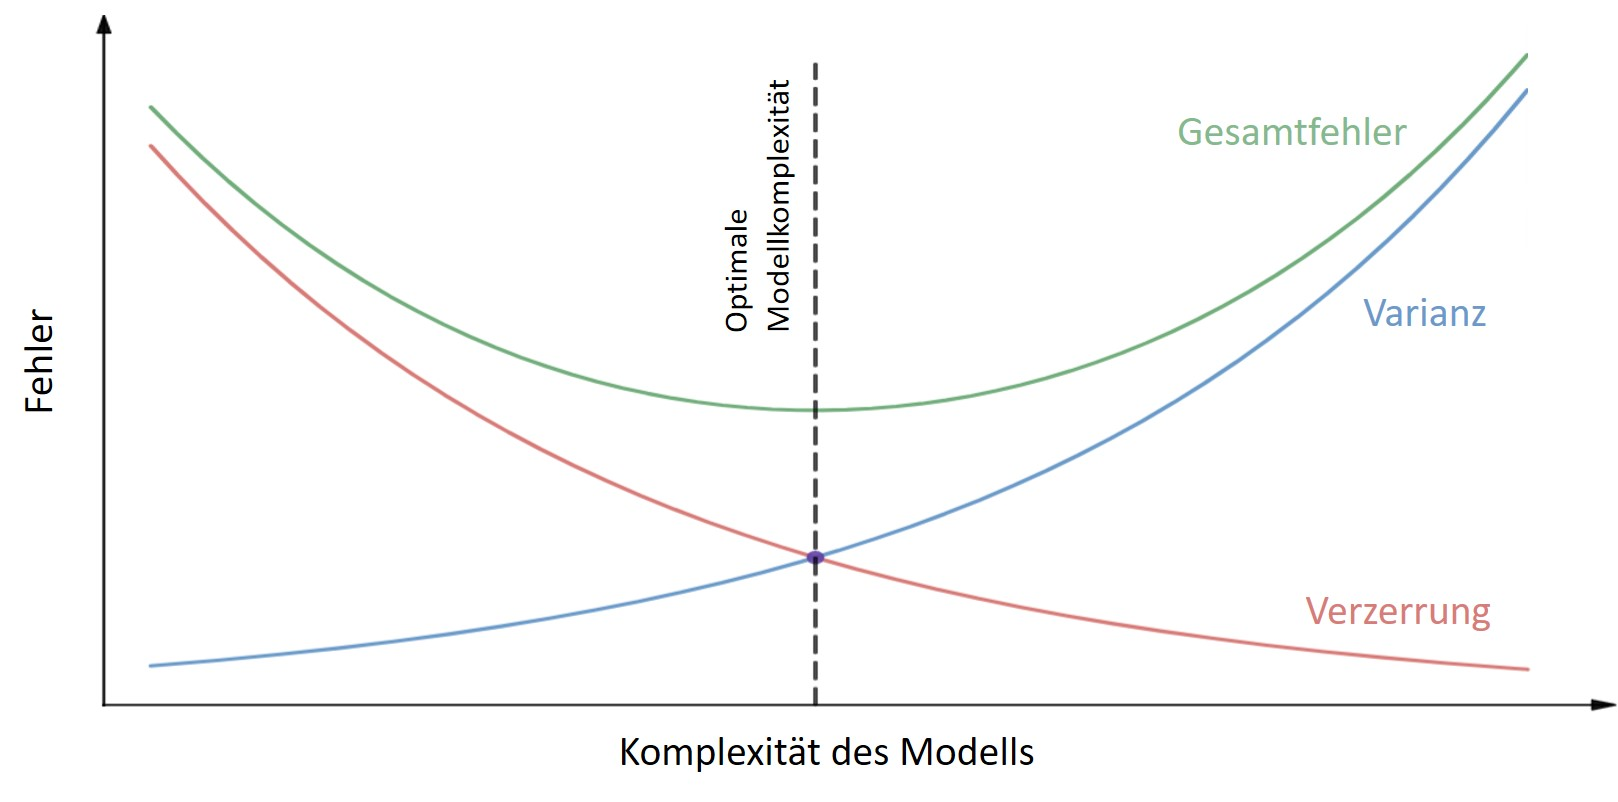
\includegraphics[width = 0.9\textwidth]{figures/bias_variance_tradeoff_labeled.jpg}
\caption{Verzerrung-Varianz-Dilemma}
\label{bias_variance_tradeoff}
\end{figure}

\subsection{Lineare Regression}

Bei der Regressionsanalyse werden Zusammenhänge zwischen
mehreren Merkmalen untersucht. Man versucht eine unabhängige Variable $Y$ durch eine oder mehrere abhängige Variablen $X_1, \ldots, X_p$ zu erklären. Ein lineares Regressionsmodell hat also die Form
\begin{align}
\label{linear_model}
f(X) = \beta_0 + \sum_{j=1}^p X_j\beta_j
\end{align}
wobei $\beta_j$ die Regressionskoeffizienten sind. Bei der Verwendung dieses Modells nehmen wir an, dass die Regressionsfunktion $\text{E}(Y|X)$ linear ist bzw. ein lineares Modell eine geeignete Approximation ist \cite{hastie_elements}.

Typischerweise verfügen wir über eine Menge von Trainingsdaten $(x_1, y_1), \ldots, (x_n, y_n)$. Jedes $x_i = (x_{i1}, \ldots, x_{ip})^{\top}$ stellt eine Beobachtung dar, die wir für die Schätzung der Parameter $\beta_j$ benutzen. Die bekannteste Methode für diesen Zweck ist sicherlich die \textit{Methode der kleinsten Quadraten} (Englisch: \textit{(Ordinary) Least Squares}), in welcher wir $\beta = (\beta_0, \ldots, \beta_p)^{\top}$ so wählen, dass die Summe der Residuenquadrate (Englisch: \textit{Residual Sum of Squares (RSS)} minimiert wird. Wir definieren
\begin{align}
\label{RSS}
\text{RSS}(\beta) & = \sum_{i=1}^{n}(y_i - f(x_i))^2\\
& = \sum_{i=1}^{n}(y_i - \beta_0 - \sum_{j=1}^p x_{ij}\beta_j)^2\nonumber\\
& = (y - \mat X \beta)^{\top}(y-\mat X \beta)\nonumber\\
& = \norm{y - \mat X \beta}_{2}^{2}\nonumber
\end{align}
und das dazugehörige Minimierungsproblem
\begin{align}
\label{least_squares}
\hat{\beta}^{\text{OLS}} = \argmin_{\beta} \text{RSS}(\beta)
\end{align}
wobei $\mat X \in \mathbb{R}^{n \times (p+1)}$ die Matrix der $x_i$ mit einer 1 an erster Stelle ist und $y = (y_1, \ldots, y_n)^{\top}$. An dieser Stelle möchten wir erwähnen, dass bei Verwendung dieser Methode keine Aussage über die Gültigkeit des Modells getroffen, sondern lediglich die beste lineare Approximation gefunden wird.

Falls $\mat X$ vollen Rang hat zeigt man leicht, dass (\ref{least_squares}) die eindeutige Lösung
\begin{align}
\hat{\beta}^{\text{OLS}} = (\mat X^{\top}\mat X)^{-1}\mat X^{\top} y
\end{align}
besitzt. Die Zielgröße $y$ ergibt sich dann durch
\begin{align}
\hat{y} = \mat X \hat{\beta}^{\text{OLS}} = \mat X (\mat X^{\top}\mat X)^{-1}\mat X^{\top} y
\end{align}
Die Matrix $\mat P = \mat X (\mat X^{\top}\mat X)^{-1}\mat X^{\top}$ haben wir bereits in Abschnitt \ref{orthogonality} kennengelernt. Sie projiziert $y$ orthogonal auf den durch die Spalten von $\mat X$ aufgespannten Unterraum. Dies ermöglicht eine geometrische Interpretation der linearen Regression.

Wenn $\mat X$ keinen vollen Rang hat, ist die Lösung von (\ref{least_squares}) nicht mehr eindeutig. Dieser Art Probleme ereignen sich häufig in der Bild- und Signalanalyse, bei welcher wir häufig über mehr Variablen als Beobachtungen verfügen. Um ein gewünschtes Verhalten der Regression zu gewährleisten, bestehen verschiedene Möglichkeiten der Filterung oder Regularisierung. In letzterem Fall versehen wir den Regressionsterm mit sog. \textit{Straftermen}, welche eine bedeutende Rolle in den folgenden Kapitel spielen werden. Wir möchten diese mithilfe der linearen Regression einführen. Die Effekte der Strafterme können aber auf andere verallgemeinerte lineare Modelle übertragen werden. 

Die von uns eingeführten Strafterme werden vor allem eine Schrumpfung der Regressionskoeffizienten verursachen. Daher möchten wir zunächst motivieren, in welchen Situationen eine derartige Regularisierung hilfreich sein kann.
\begin{itemize}
\item Vorhersagegenauigkeit: Besonders in $p > n$-Fällen neigt ein lineares Regressionsmodell häufig zu einer Überanpassung an die Trainingsdaten. Um die Vorhersagegenauigkeit für ungesehene Testdaten zu verbessern, kann eine Erhöhung des Bias im Sinne des Verzerrung-Varianz-Dilemmas sinnvoll sein. Dies können wir beispielsweise dadurch erreichen, dass wir die Regressionskoeffizienten verkleinern oder sogar auf 0 setzen.
\item Interpretation: Eine hohe Anzahl an Variablen, die in das Modell einfließen erschwert unzweifelhaft eine Interpretation. Daher kann es von Vorteil sein nur einen Teil der Variablen für das Modell auszuwählen. Optimalerweise selektiert man solche, die eine möglichst genaue Vorhersage ermöglichen.
\end{itemize}

Ein naheliegender Ansatz zur Lösung dieser Probleme wäre es zu versuchen, eine $k$-Teilmenge der Variablen zu finden, die eine minimale Summe der Residuenquadrate aufweist. In \cite{hastie_elements} werden verschiedene Methoden zur exakten und approximativen Berechnung dieser Teilmenge beschrieben. Nicht immer wird die Genauigkeit der Vorhersagen durch Verwendung dieses Ansatzes besser. Dies liegt vor allem daran, dass Variablen für das Modell entweder ausgewählt oder verworfen werden. Daher beschäftigen wir uns nun mit Methoden, die eine kontinuierliche Schrumpfung der Regressionskoeffizienten erlauben.

\subsection{Ridge Regression}

Zu diesem Zweck kann die \textit{Tikhonov Regularisierung}, die auch unter dem Namen \textit{Ridge Regression} bekannt ist, genutzt werden. Mithilfe eines \textit{Ridge Strafterms} opfern wir einen Teil des Bias für verbesserte Vorhersagen im Sinne des Verzerrung-Varianz-Dilemmas. Wir formulieren das Ridge Regression Problem in der Lagrange Form
\begin{align}
\label{ridge_regression}
\hat{\beta}^{\text{ridge}} = \argmin_{\beta} \sum_{i=1}^{n}(y_i - \beta_0 - \sum_{j=1}^p x_{ij}\beta_j)^2 + \lambda_2\sum_{j=1}^p \beta_j^2
\end{align}
wobei $\lambda_2 \geq 0$ ein Parameter ist, der die Stärke der Schrumpfung der Regressionskoeffizienten kontrolliert. Je größer $\lambda_2$, desto stärker ist die Schrumpfung der $\beta_j$. Durch die Einführung des $\ell_2$-Strafterms garantiert (\ref{ridge_regression}) auch für $p > n$ eine eindeutige Lösung. Da $\beta_0$ nicht im Strafterm vorkommt, schätzen wir zunächst $\beta_0 = \bar{y} = \frac{1}{n}\sum_{i=1}^{n} y_i$ und zentrieren die Eingaben $x_{ij} = x_{ij} - \bar{x}_j$. Die eindeutige Lösung der zentrierten Version von (\ref{ridge_regression}) ist dann durch
\begin{align}
\hat{\beta}^{\text{ridge}}  = (\mat X^{\top} \mat X + \lambda_2\mat{I})^{-1}\mat{X}^{\top}y
\end{align}
gegeben, wobei $\beta = (\beta_1, \ldots, \beta_p)$ und $\mat{X} \in \mathbb{R}^{n \times p}$ die Matrix der $x_i$. Die durch die Ridge Regression erzeugten Koeffizienten sind also um den Faktor $\frac{1}{1+\lambda_2}$ gegenüber denen der klassischen linearen Regression skaliert. Eine Dünnbesetzung der Koeffizienten wird also erst für $\lambda_2 \to \infty$ erreicht.

\subsection{LASSO}
\label{lasso}

Um eine bessere Interpretation des Modells zu ermöglichen, versucht man bei der \textit{Lasso} Regression eine Lösung zu finden, bei welcher viele Koeffizienten gleich Null sind. Das Lasso wurde erstmals von Tibshirani in \cite{tibshirani_lasso} eingeführt und ist in der Signalanalyse unter dem Namen \textit{Basis Pursuit} \cite{chen} bekannt. Mathematisch gesehen erreichen wir eine Dünnbesetzung durch Einbettung eines $\ell_1$-Strafterms.
\begin{align}
\label{lasso_formulation}
\hat{\beta}^{\text{lasso}} = \argmin_{\beta} \sum_{i=1}^{n}(y_i - \beta_0 - \sum_{j=1}^p x_{ij}\beta_j)^2 + \lambda_1\sum_{j=1}^p \left|\beta_j\right|
\end{align}
Es wird also im Vergleich zu (\ref{ridge_regression}) lediglich die $\ell_2$-Norm durch eine $\ell_1$-Norm ausgetauscht. Bevor wir uns mit der Lösung dieses Problems beschäftigen, möchten wir erklären, warum die $\ell_1$-Norm eine Dünnbesetzung hervorruft. Zunächst geben wir eine geometrische Erklärung, welche in Abbildung \ref{lasso_ridge_regression_figure} zu sehen ist. Dort sind die $\ell_1$- und $\ell_2$-Beschränkungen, sowie die Höhenlinien der RSS-Funktion in zwei Dimensionen aufgezeichnet. Die optimalen Koeffizienten von Ridge und Lasso Regression ergeben sich nun aus dem Schnittpunkt der Höhenlinien mit der Begrenzung der jeweiligen Norm. Im Falle der $\ell_1$-Norm ist dieser Schnittpunkt mit einer hohen Wahrscheinlichkeit an eine der Ecken, so dass einer der beiden Koeffizienten auf Null gesetzt wird. Im Gegensatz dazu ist die Wahrscheinlichkeit bei einer $\ell_2$-Begrenzung sehr gering, da keine Ecken vorhanden sind. Somit kommt jeder Randpunkt der Begrenzung als Schnittpunkt in Frage und es wird keine Dünnbesetzung, sondern lediglich eine kontinuierliche Schrumpfung der Koeffizienten hervorgerufen. Dieser Effekt verstärkt sich in höheren Dimensionen.

\begin{figure}
\centering
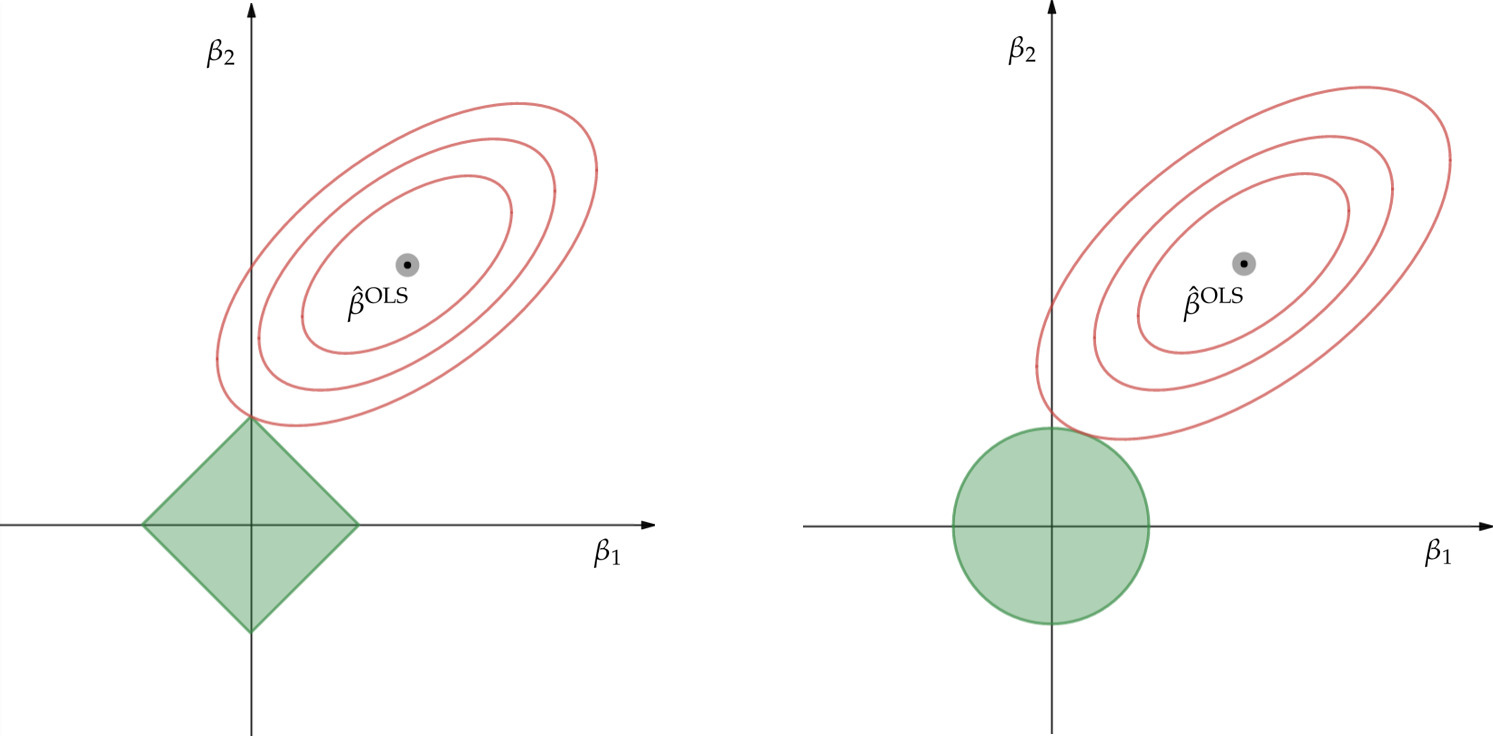
\includegraphics[width = 0.9\textwidth]{figures/lasso_ridge_regression.jpg}
\caption{Die Abbildung zeigt die Beschränkungen der $\ell_1$-Norm (links) und der $\ell_2$-Norm (rechts) zusammen mit den Höhenlinien der RSS-Funktion im $\mathbb{R}^2$. Verdeutlicht wird hier die geometrische Findung von $\hat{\beta}^{\text{lasso}}$ (links) und $\hat{\beta}^{\text{ridge}}$ (rechts). (Abbildung basiert auf \cite{hastie_elements})}
\label{lasso_ridge_regression_figure}
\end{figure}

An dieser Stelle kann man auf den Gedanken kommen, andere Strafterme zu verwenden, welche bei geometrischer Betrachtung die Wahrscheinlichkeit erhöhen eine Dünnbesetzung der Koeffizienten hervorzurufen. So kann man zum Beispiel die $\ell_q$-Normen als Strafterm für Werte $q < 1$ in Betracht ziehen. In Abbildung \ref{norm_figure} sind die Begrenzungen der $\ell_q$-Normen für verschiedene Werte von $q$ eingezeichnet. Für $q \rightarrow 0$ entstehen sternförmige Höhenlinien, welche immer weiter zum Ursprung gedrückt werden. Somit wird es immer wahrscheinlicher, dass die Höhenlinien der RSS-Funktion eine Ecke treffen und wir dünnbesetzte Koeffizienten erhalten. Daher kann man folgendes Berechnungsproblem definieren
\begin{align}
\label{sparse_regression}
\hat{\beta}^{\text{sparse}} = \argmin_{\beta} \sum_{i=1}^{n}(y_i - \beta_0 - \sum_{j=1}^p x_{ij}\beta_j)^2 + \lambda_q\sum_{j=1}^p \left|\beta_j\right|^q
\end{align}
Leider ist dies nur in der Theorie ein guter Ansatz. Das Problem liegt nicht im Effekt der verschiedenen Strafterme, sondern in der Berechnung. Für $q < 1$ ist (\ref{sparse_regression}) ein nicht-konvexes Optimierungsproblem, da $\norm{\cdot}_q$ keine Norm gemäß Definition \ref{norm} ist. Im Extremfall der $\ell_0$-\q{Norm} wird (\ref{sparse_regression}) sogar NP-schwer \cite{foucart}. Somit besteht keine effiziente Methode zur Berechnung von $\hat{\beta}^{\text{sparse}}$ zur Verfügung. Der Wert $q = 1$ ist eine Art Kompromisslösung, die einerseits effizient zu berechnen ist und andererseits noch immer eine dünnbesetzte Lösung liefert.

\begin{figure}
\centering
	\begin{subfigure}{0.2\textwidth}
	\centering
	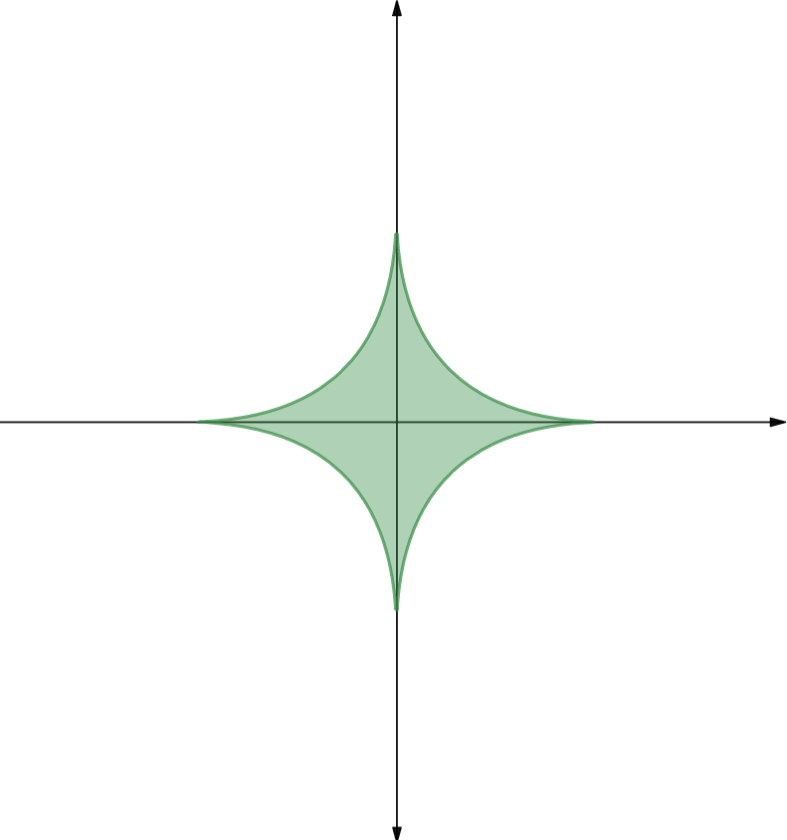
\includegraphics[width = \textwidth]{figures/norm_0_5.png}
	\label{norm_0_5_figure}
	\caption*{$q = 0.5$}
	\end{subfigure} \hspace{0.5cm}
	%	
	\begin{subfigure}{0.2\textwidth}
	\centering
	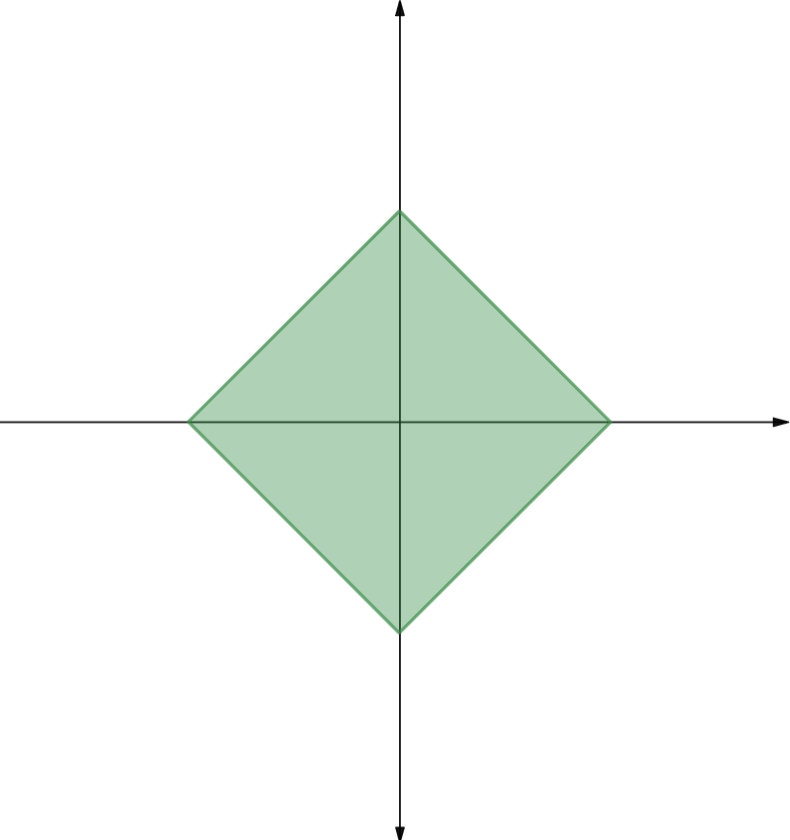
\includegraphics[width = \textwidth]{figures/norm_1.png}
	\label{norm_1_figure}
	\caption*{$q = 1$}
	\end{subfigure}\hspace{0.5cm}
	%
	\begin{subfigure}{0.2\textwidth}
	\centering
	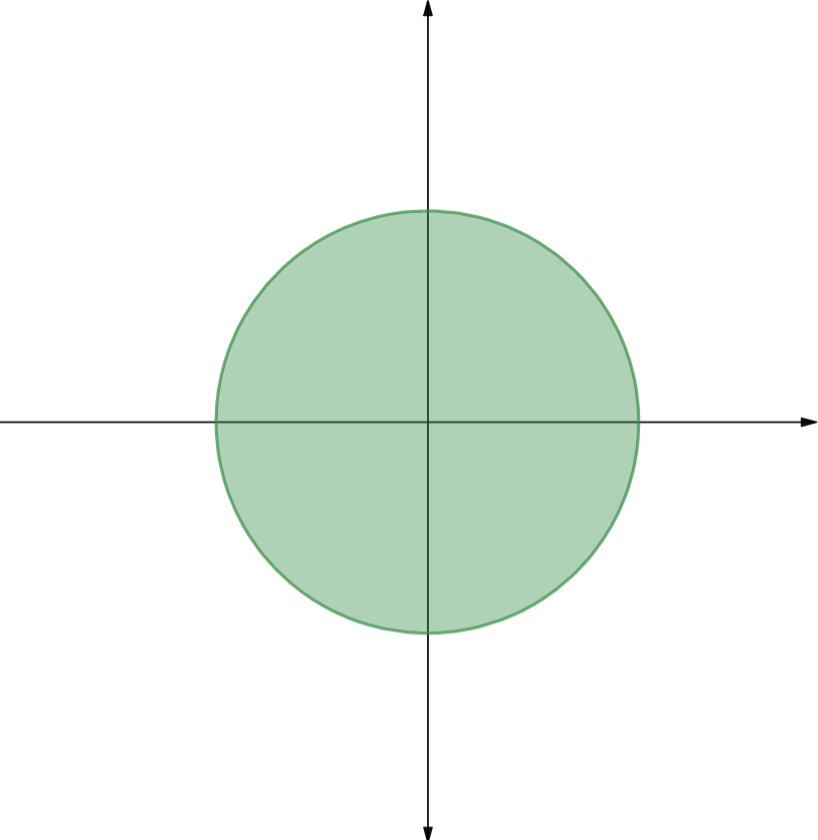
\includegraphics[width = \textwidth]{figures/norm_2.png}
	\label{norm_2_figure}
	\caption*{$q = 2$}
	\end{subfigure}\hspace{0.5cm}
	%
	\begin{subfigure}{0.2\textwidth}
	\centering
	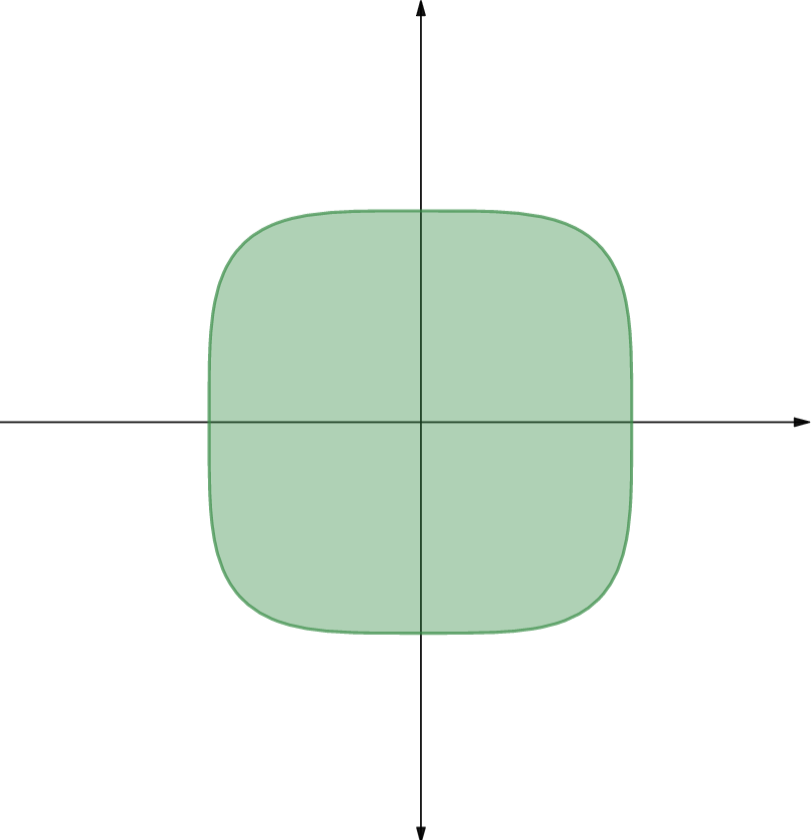
\includegraphics[width = \textwidth]{figures/norm_4.png}
	\label{norm_4_figure}
	\caption*{$q = 4$}
	\end{subfigure}

\caption{Die Abbildung zeigt die Begrenzungen der $\ell_q$-Norm im $\mathbb{R}^2$ für verschiedene Werte von $q$, also die Mengen $\{x \in \mathbb{R}^2 \colon \norm{x}_{q} \leq c \}$. (Abbildung basiert auf \cite{hastie_elements})}
\label{norm_figure}
\end{figure}

Um eine mathematisch gründliche Erklärung für die Dünnbesetzung zu liefern, wenden wir uns der Lösung von (\ref{lasso_formulation}) zu. Falls die Spalten von $\mat X$ orthonormal sind, ergibt sich eine explizite Lösung
\begin{align}
\hat{\beta}_j^{\text{lasso}} = \text{sign}(\hat{\beta}_j^{\text{OLS}}) \left(\left|\hat{\beta}_j^{\text{OLS}}\right| - \frac{\lambda_1}{2}\right)_{+}
\end{align}
wobei $(\cdot)_+ = max(\cdot, 0)$ ist. Der Beweis kann in \cite{murphy} nachgelesen werden. Die Lösung ist also durch den sog. \textit{soft thresholding operator} gegeben, welcher durch
\begin{align}
\text{soft}_{\delta}(x) = \text{sign}(x)(|x| - \delta)_+
\end{align}
definiert wird. Dieser ist in Abbildung \ref{thresholding_figure} im Gegensatz zum hard-thresholding Operator dargestellt. Nun sind wir auch in der Lage zu verstehen, warum Tibshirani \cite{tibshirani_lasso} den Begriff Lasso eingeführt hat, welcher für \textit{Least absolute selection and shrinkage operator} steht. Es werden zunächst alle Koeffizienten in $\hat{\beta}^{\text{OLS}}$, die kleiner als $\frac{\lambda_1}{2}$ sind, auf $0$ gesetzt und die Verbliebenden anschließend im Betrag um $\frac{\lambda_1}{2}$ geschrumpft. 

\begin{figure}
\centering
	\begin{subfigure}{0.4\textwidth}
	\centering
	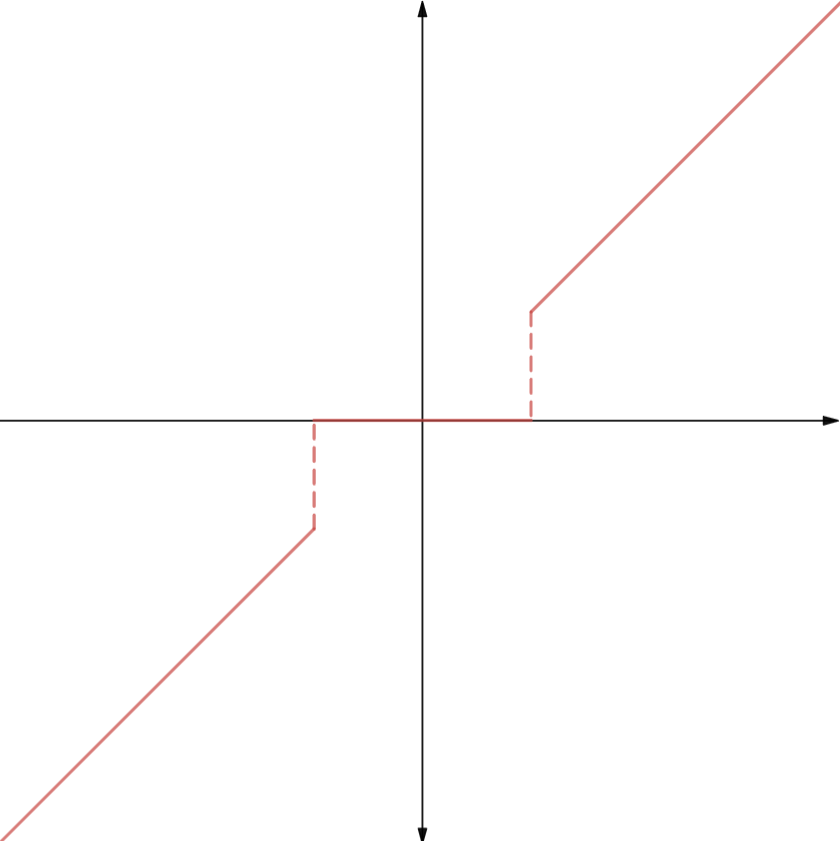
\includegraphics[width = \textwidth]{figures/hard_thresholding.png}
	\label{hard_thresholding}
	\end{subfigure}\hspace{1cm}
	%	
	\begin{subfigure}{0.4\textwidth}
	\centering
	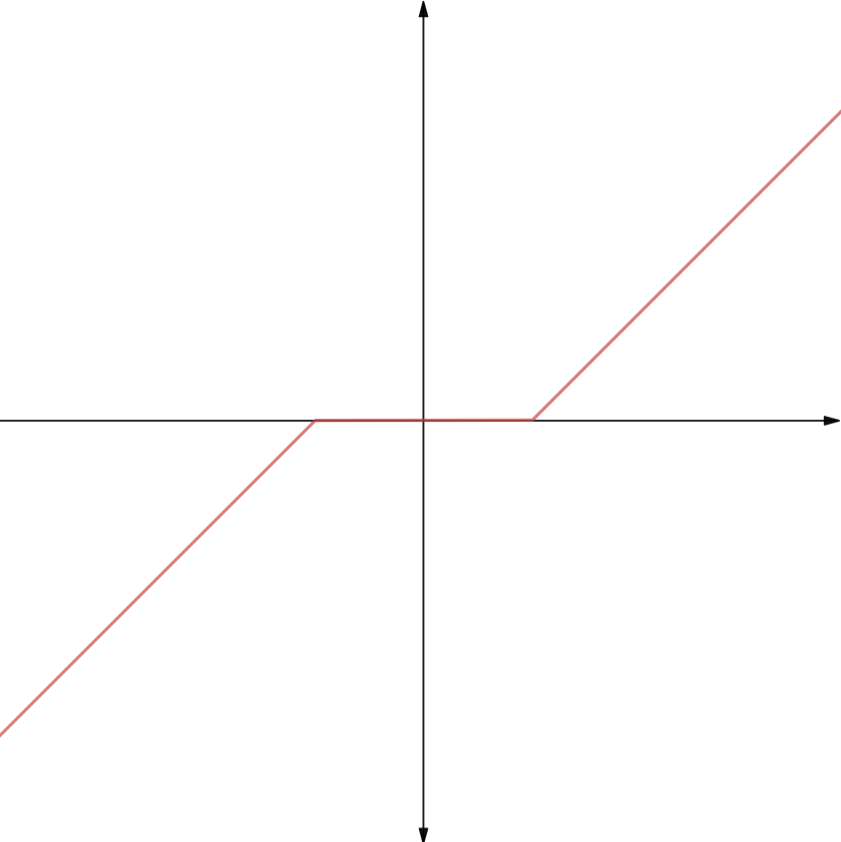
\includegraphics[width = \textwidth]{figures/soft_thresholding.png}
	\label{soft_thresholding}
	\end{subfigure}
\caption{Die Abbildung zeigt die beiden Operationen soft und hard thresholding}
\label{thresholding_figure}
\end{figure}

Für den allgemeinen Fall wird (\ref{lasso_formulation}) mithilfe von Näherungsverfahren gelöst. Da $\norm{\beta}_1$ nicht differenzierbar ist wenn $\beta_j = 0$, sind wir mit einem nicht glattem Optimierungsproblem konfrontiert. Seit der Problemformulierung wurde eine Vielzahl an Algorithmen entwickelt bzw. adaptiert, die eine numerische Lösung liefern. Dazu gehören Least-angle Regression (LARS) \cite{efron_lars}, Koordinaten-Abstiegsverfahren \cite{friedman}, Subdifferential-Methoden und  Näherungs-Gradientenverfahren \cite{yang, vandenberghe}. Letztere sind eine natürliche Erweiterung von Gradientenverfahren falls die Zielfunktion nicht differenzierbar ist. In Abschnitt \ref{elastic_net}, werden wir auf ein Koordinaten-Abstiegsverfahren näher eingehen.

Es stellt sich heraus, dass das Lasso zwei wesentliche Nachteile besitzt. Falls es im Datensatz Gruppen stark korrelierter Variablen gibt, tendiert die Methode dazu nur eine Variable je Gruppe statt die Gruppe als Ganzes auszuwählen. Zum Beispiel bei der Suche nach Genen, welche mit einer bestimmten Krankheit verbunden sind, ist man aber daran interessiert, alle assoziierten Koeffizienten zu finden. Darüber hinaus führt dieser Effekt zu verschlechterten Vorhersagen. Um diesem Problem zu entgegnen kann man das sog. \textit{Group Lasso} verwenden \cite{yuan}, bei welcher man zuvor Gruppen im Datensatz festlegen kann. Der im Zuge dieser Arbeit aber wichtigere Nachteil ist, dass das Lasso für $p > n$ Datensätze maximal $n$ Variablen selektieren kann. Da $\mat X$ in diesem Fall maximal Rang $n$ hat, können wir $y$ mithilfe von $n$ Variablen perfekt vorhersagen. Das Lasso wählt dann die $n$ Variablen, welche $\lambda_1\norm{\beta}_1$ minimieren. Für moderne Datensätze mit $p \gg n$ ist es aber oft nicht ausreichend, nur $n$ von null verschieden Koeffizienten zuzulassen.

\subsection{Elastic Net}
\label{elastic_net}

Damit im Fall $p > n$ mehr als $n$ Variablen selektiert werden können, betrachten wir eine Verallgemeinerung von Lasso und Ridge Regression. Durch die Einbettung einer $\ell_1$ und $\ell_2$-Norm erhalten wir das sog. \textit{Elastic Net} \cite{zou_elasticnet}.
\begin{align}
\label{elastic_net_formulation}
\hat{\beta}^{\text{en}} = \argmin_{\beta} \norm{y - \mat X \beta}_2^2 + \lambda_2 \norm{\beta}_{2}^{2} + \lambda_{1,j} \norm{\beta}_{1}
\end{align}
Wie zuvor wird durch den $\ell_1$-Strafterm ein dünnbesetztes Modell generiert. Dagegen fördert der $\ell_2$-Strafterm den Gruppeneffekt, stabilisiert den $\ell_1$ Regularisierungspfad und lässt eine beliebige Anzahl zu selektierender Variablen zu. Um eine doppelte Schrumpfung der Koeffizienten zu vermeiden, kann das Elastic Net mit dem Faktor $(1 + \lambda_2)$ korrigiert werden. 

Ähnlich wie bei der Lasso Regression kann nur dann eine explizite Lösung von (\ref{elastic_net_formulation}) angegeben werden, falls die Spalten von $\mat X$ orthonormal sind. Daher wurden verschiedene Näherungsverfahren für eine numerische Lösung vorgeschlagen. Dazu gehören beispielsweise LARS-EN \cite{zou_elasticnet}, welches auf dem LARS Algorithmus für das Lasso basiert, und ein Koordinatenabstiegsverfahren \cite{friedman}. Letzteres werden wir in unseren Implementierung in Kapitel \ref{implementation} für ein Subproblem nutzen.

https://stats.stackexchange.com/questions/123672/coordinate-descent-soft-thresholding-update-operator-for-lasso

We propose an efficient algorithm called LARS-EN to solve the elastic net efficiently, which is
based on the recently proposed algorithmLARSof Efron et al. (2004). They proved that, starting
from zero, the lasso solution paths grow piecewise linearly in a predictable way. They proposed
a new algorithm called LARS to solve the entire lasso solution path efficiently by using the same
order of computations as a single OLS fit

Die Implementierung des Elastic Nets in scikit-learn \cite{scikit_learn} beruht auf einer anderen, aber sehr ähnlichen mathematischen Formulierung
\begin{align}
\label{elastic_net_python}
\hat{\beta}^{\text{en}} = \argmin_{\beta} \frac{1}{2n} \norm{y - \mat X \beta}_2^2 + \alpha \gamma \norm{\beta}_{1} + \frac{1}{2}\alpha (1-\gamma) \norm{\beta}_{2}^2
\end{align}
wobei $n$ die Anzahl an Beobachtungen im Datensatz und $\gamma \in [0,1]$ das Verhältnis zwischen $\ell_1$- und $\ell_2$-Norm ist. Mit $\gamma = 0$ reduziert sich (\ref{elastic_net_python}) auf Ridge und für $\gamma = 1$ auf die Lasso Regression. Somit können wir durch $\gamma$ das Verhältnis der beiden Regressionen kontrollieren und durch $\alpha$ die Stärke der Bestrafung. Setzt man 
\begin{align}
 \alpha = \frac{2\lambda_2 + \lambda_1}{2n} \quad \text{und} \quad \gamma = \frac{\lambda_1}{2\lambda_2 + \lambda_1}
\end{align}
entspricht (\ref{elastic_net_python}) unser ursprünglich formulierten Problem. An dieser Stelle möchten wir anmerken, dass bei dieser Implementierung nicht die Möglichkeit besteht, die Koeffizienten unterschiedlich zu bestrafen im Gegensatz zu (\ref{elastic_net_formulation}).

\subsection{Vergleich der Regressionsmethoden}
\label{comparison_linear_models}

Zur Veranschaulichung der oben eingeführten Methoden werden wir diese zur Anwendung bringen. Dabei greifen wir auf einen durch scikit-learn \cite{scikit_learn} bereitgestellten Datensatz, der erstmals durch \cite{efron_lars} öffentlich gemacht worden ist, zurück. In diesem wurden für $n = 442$ Diabetes Patienten $p=10$ verschiedene Variablen gemessen. Dazu gehören Alter (AGE), Geschlecht (SEX), Body Mass Index (BMI), Blutdruck (BP) und verschiedene Blutproben (Serum Measurements). Die Zielgröße $y$ enthält Werte für den Krankheitsfortschritt ein Jahr nach Behandlungsbeginn. Ein Ausschnitt des Datensatzes befindet sich in Tabelle \ref{diabetes_data_set}.

\begin{table}
\centering
\begin{tabular}[c]{c|cccccccccc|c}
& \thead{AGE} & \thead{SEX} & \thead{BMI} & \thead{BP} & \multicolumn{6}{c|}{\ldots \thead{Serum Measurements} \ldots} & \thead{Response}\\
\thead{Patient} & \thead{x1} & \thead{x2} & \thead{x3} & \thead{x4} & \thead{x5} & \thead{x6} & \thead{x7} & \thead{x8} & \thead{x9} & \thead{x10} & \thead{y}\\
\hline
1 & 59 & 2 & 32.1 & 101 & 157 & 93.2 & 38 & 4 & 4.9 & 87 & 151\\
2 & 48 & 1 & 21.6 & 87 & 183 & 103.2 & 70 & 3 & 3.9 & 69 & 75\\
3 & 72 & 2 & 30.5 & 93 & 156 & 93.6 & 41 & 4 & 4.7 & 85 & 141\\
4 & 24 & 1 & 25.3 & 84 & 198 & 131.4 & 40 & 5 & 4.9 & 89 & 206\\
\vdots & \vdots & \vdots & \vdots & \vdots & \vdots & \vdots & \vdots & \vdots & \vdots & \vdots & \vdots\\
441 & 36 & 1 & 30.0 & 95 & 201 & 125.2 & 42 & 5 & 5.1 & 85 & 220\\
442 & 36 & 1 & 19.6 & 71 & 250 & 133.2 & 97 & 3 & 4.6 & 92 & 57\\
\end{tabular}
\caption{Diabetes Datensatz \cite{efron_lars, diabetes_data}}
\label{diabetes_data_set}
\end{table}

Schrumpfung bei Ridge Regression kontinuierlich.
Die Ergebnisse der Regressionen können in Abbildung \ref{regression_coefficients} und \ref{regression_coefficients_mse} eingesehen werden. 

\begin{figure}
\centering
	\begin{subfigure}{0.9\textwidth}
	\centering
	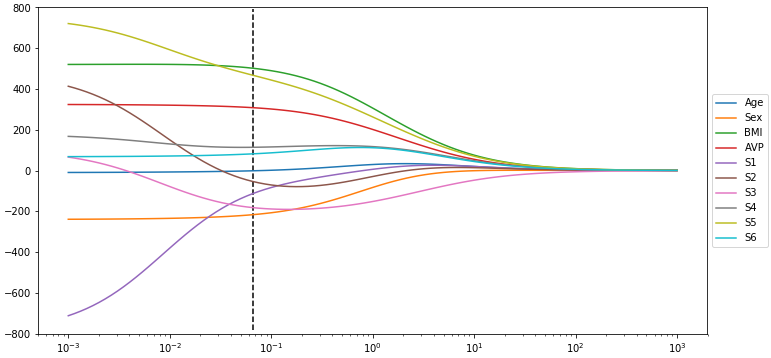
\includegraphics[width = \textwidth]{figures/ridge_regression_coefficients_cv.png}
	\label{ridge_regression_coefficients}
	\vspace{-0.5cm}
	\caption{Ridge Regression}
	\vspace{0.5cm}
	\end{subfigure}
	%	
	\begin{subfigure}{0.9\textwidth}
	\centering
	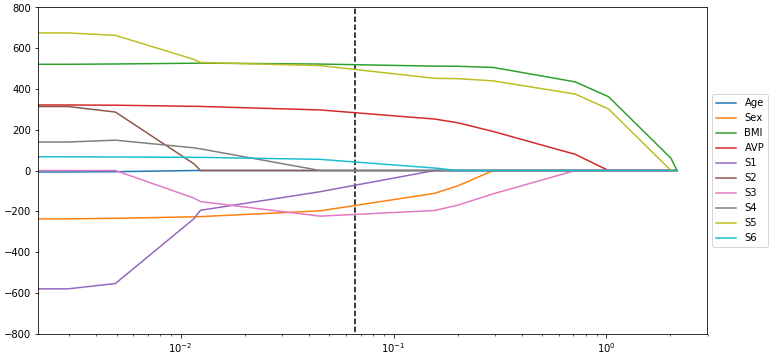
\includegraphics[width = \textwidth]{figures/lasso_regression_coefficients_cv.png}
	\label{lasso_regression_coefficients}
	\vspace{-0.5cm}
	\caption{Lasso Regression}
	\vspace{0.5cm}
	\end{subfigure}
	%
	\begin{subfigure}{0.9\textwidth}
	\centering
	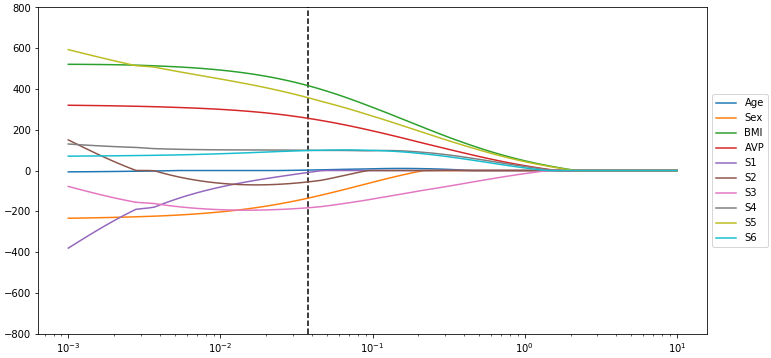
\includegraphics[width = \textwidth]{figures/elastic_net_coefficients_cv.png}
	\label{elastic_net_coefficients}
	\vspace{-0.5cm}
	\caption{Elastic Net, $\gamma = 0.98$}
	\end{subfigure}
\caption{Schrumpfung der Koeffizienten für verschiedene Regressionsmethoden bei Erhöhung des jeweiligen Regularisierungsparameters. Die vertikalen Linien stellen den Wert des jeweiligen Parameters dar, der durch ein 10-faches Kreuzvalidierungsverfahren bestimmt worden ist. (Erstellt mit scikit-learn)}
\label{regression_coefficients}
\end{figure}

\begin{figure}
\centering
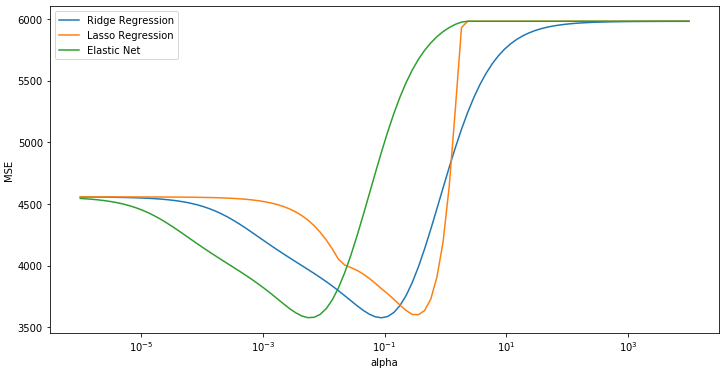
\includegraphics[width=0.9\textwidth]{figures/regression_coefficients_mse.png}
\label{regression_coefficients_mse}
\caption{Selektion des Modells gemäß der mittleren quadratischen Abweichung für Ridge, Lasso und Elastic Net Regression}
\end{figure}


%----------------------------------------------------------------------------------------
%	Signaltheorie
%----------------------------------------------------------------------------------------


\section{Signaltheorie}
\label{signal_processing}

\subsection{Fouriertransformation}
\subsection{Nyquist-Shannon Abtasttheorem}